%!TEX root = ../cluster_semi.tex
\begin{figure*}
  \centering
  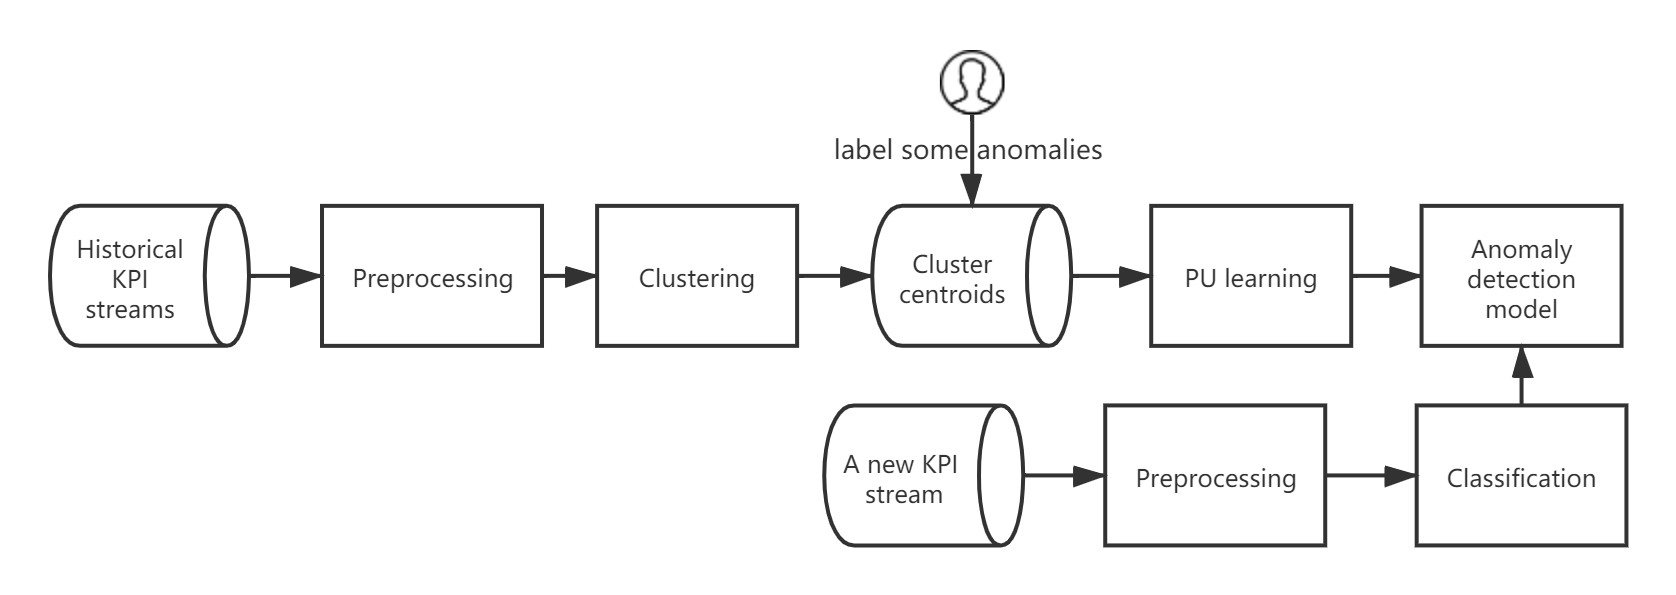
\includegraphics[width=0.9\linewidth]{ADS_Journal/PU figures/Whole Framework (1).png}
  \caption{
    The framework of~\name{}
  }
  \label{fig:overview}
  \vspace{-6 mm}
\end{figure*}

\section{Framework of PUAnomaly}
\label{sec:algorithm}
In address to solve the challenge of large-scale KPI stream anomaly detection, we propose \name{}, an anomaly detection framework based on PU learning for time series.
% To address the challenges of the high cost of model training and anomalies labeling, we propose \name{}, an anomaly detection framework based on PU learning for time series. Figure~\ref{fig:overview} shows the overall workflow of \name{}. 
\textcolor{red}{To solve the first challenge we adopt clustering which divides the historical KPIs into several clusters and train a final model by using the new KPI and the KPI closest to its centroid.
As for the second challenge, we create a new labeling strategy of active learning to validate the highly reliable positive samples, which significantly improves the efficiency of active learning.}

% Fig.~\ref{fig:overview} give an overview of our algorithm, consists of offline clustering component and online training component. The key techniques are clustering and semi-supervised learning.
 
 For existing/historical KPI streams, \name~preprocesses them with filling missing points and standardization firstly. Next, \name~clusters the preprocessed KPI streams and extract features of the cluster centroids. Afterward, based on the features of each cluster centroid, \name~exploits PU learning with active learning to obtain enough credible labeled samples. 
 As for a newly emerging KPI stream, \name~preprocesses it and classifies it into one of the existing clusters. Then, \name~assigns PU learned samples that belong to its cluster to it and train a corresponding anomaly model for it by semi-supervised learning using its unlabeled samples and PU learned samples.

%这里要不要删掉呢~
% \textcolor{red}{
% As for a newly emerging KPI stream, \name~preprocesses it and classifies it into one of the existing clusters. Based on the corresponding anomaly detection model, we can detect the anomalies of the newly emerging KPI stream.}

We will describe more details about \name~ in the following sections.
\par


\subsection{Preprocessing}
\label{subsubsec:preprocessing}
Because of monitoring system malfunctions and/or operator misconfigurations, the KPI stream could occasionally miss some points \cite{ADSarticle}, which could change the mode of the KPI stream. 
For example, if missing points are ignored, incorrect features may be obtained in subsequent feature extraction, which will affect the performance of the whole framework.
Therefore, we fill these missing points using linear interpolation following~\cite{lirobust}.
\par
Besides, since different KPI corresponding to different performance indicators usually have different amplitude and length scales, to make these KPI streams comparable, we also standardize KPI streams with Z-score.
This way, different KPI streams could be clustered based on their shapes in \ref{subsubsec:clustering}, rather than the absolute values of amplitudes and/or length scales.

\subsection{Clustering}
\label{subsubsec:clustering}
As discussed in Section~\ref{sec:introduction}, a lot of KPI streams are similar because of their implicit association, therefore we could use a clustering method to cluster many KPI streams into clusters to reduce the workload by several orders of magnitude. In our experiment, we clustered 126 KPIs into 9 clusters. \name~adopts ROCKA~\cite{lirobust} to cluster the preprocessed historical KPI streams into a few clusters and obtains a centroid KPI stream for each cluster by comparing the shape-based distance(SBD) distance between each KPI and the centroid of the cluster.
As for a newly KPI stream, it will be classified into the nearest cluster by calculating the shape-based distance (SBD) from each existing cluster centroid KPI stream.
% When a newly KPI stream emerging, it will be classified into the nearest cluster by preprocessing as well as calculating the shape-based distance (SBD) from each existing cluster centroid.

\subsection{Feature Extraction}
\label{subsubsec:feature_extraction}
The raw data point in the KPI stream cannot show the information about whether it is an anomaly or not directly, so \name~extracts the features of the KPI streams by converting each data point to a set of features, which indicate the likelihood that the data point is anomalous.
% The centroid of each cluster represents the cluster's characteristics, therefore we extract the features of the KPI stream on each cluster centroid to build the final model. When there emerging a new data point, we also convert it into a set of features.
The features extracted by \name~could be categorized into two groups: temporal features  and forecasting error features.
\par
\subsubsection{Temporal Features}
\label{subsubsubsec:temporal_features}
In general, when the value in a KPI stream changes dramatically in a short period, it is likely to be an anomaly. Therefore, \name~extracts some temporal features (as shown in Table \ref{tab:temporal_feature}) to evaluate the changes of KPI stream in a short time.
In this part, we compute the slope, standard deviation, coefficient of variation, and so on. Some of these features are calculated based on time points to evaluate the change of a time point, while others are calculated based on sliding windows to evaluate the change of a period of time. The length of the sliding window $w$ is taken as a parameter, which is set as 6 in our experiment and can be tuned for different scenarios and requirements.
% \usepackage{booktabs}
% Please add the following required packages to your document preamble:
% \usepackage{booktabs}
% Please add the following required packages to your document preamble:
\begin{table}[]
\caption{Temporal features extracted by \name~.}
\begin{tabular}{{|p{3cm}|p{5cm}|}}
\hline
\textbf{Feature}           & \textbf{Description}                                                                                          \\ \hline
Slope\_ratio               & Slope between two consecutive points.                                                                          \\ \hline
Sum\_ratio                 & Slope between two consecutive windows.                                                                         \\ \hline
Cv\_delta                  & Difference of coefficient of variation between two consecutive windows.                                        \\ \hline
Cv\_slope                  & Slope of coefficient of variation between two consecutive windows.                                             \\ \hline
Ping\_delta                & Difference between two consecutive points.                                                                     \\ \hline
Sum\_delta                 & Difference between two consecutive windows.                                                                    \\ \hline
Long\_time\_delta          & Difference between current point and the previous long time window.                                            \\ \hline
Long\_time\_slope          & Slope between current point and the previous long time window.                                                \\ \hline
Block\_delta               & Difference between two adjacent windows.                                                                       \\ \hline
Block\_slope               & Slope between two adjacent windows.                                                                            \\ \hline
Block\_dping\_delta        & Difference between current point and the previous window.                                                     \\ \hline
Shift\_block\_dping\_delta & Shift between current point and previous window.                                                               \\ \hline
Std                        & Standard deviation in a window.                                                                                \\ \hline
Std\_delta                 & Difference of standard deciation  between two consecutive windows.                                             \\ \hline
Max\_level\_shift          & Max trimmed mean between two consecutive windows.                                                             \\ \hline
Max\_var\_shift            & Max variance shift between two consecutive windows.                                                           \\ \hline
Max\_KL\_shift             & Max shift in Kullback-Leibler divergence between two consecutive windows.                                     \\ \hline
Lumpiness                  & Changing variance in remainder.                                                                                \\ \hline
Flatspots                  & Discretize time series values into ten equal-sized intervals. Find maximum run length within the same bucket. \\ \hline
\end{tabular}
\label{tab:temporal_feature}
\end{table}

\begin{figure*}
  \centering
  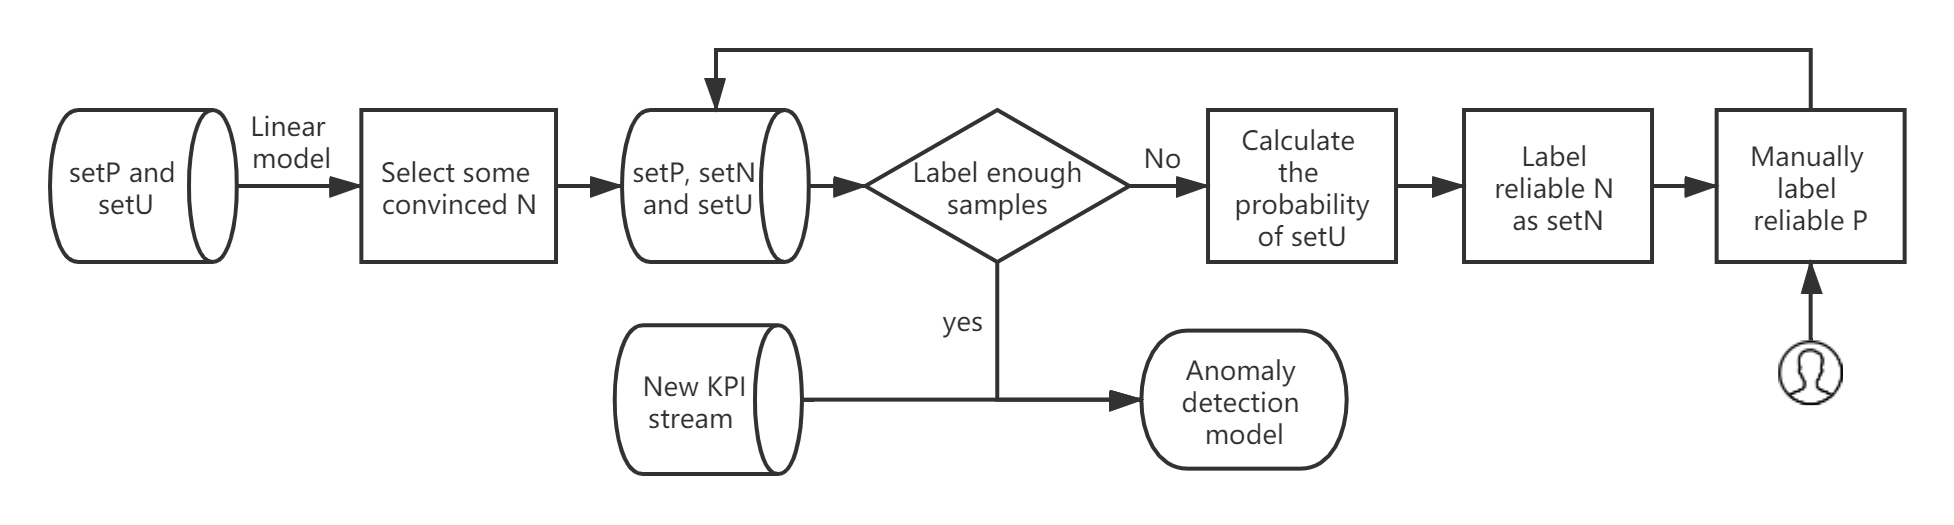
\includegraphics[width=0.9\linewidth]{ADS_Journal/PU figures/Frame of PU learning - change.png}
  \caption{
    The framework of PU learning and active learning.
  }
  \label{fig:PU learning overview}
  \vspace{-6 mm}

\end{figure*}

\subsubsection{Forecasting Error Features}
\label{subsubsubsec:forecasting_error_features}
Due to the periodicity of network service, for example, every night is usually the trough of KPI, \name~uses this to forecast the future value. If the forecasting value differs too much from the actual value, this point is could be an anomaly generally. Therefore, \name~uses some classical time series prediction models such as Holt, STL, and Holt-Winters to extract forecasting error features, which usually have less computation overhead and are easy to be interpreted.
Holt can obtain the trend of the KPI stream, Holt-Winters and STL can obtain not only the trend but also the periodic law. Therefore, \name~can predict the short term trend by Holt and the long term trend by Holt-Winters and STL,
\par Before calculating the forecasting value, we should know the period $p$ of the most dominant frequency by the Discrete Fourier Transform.
To calculate the forecasting value, we should set the length of the sliding window $w$ for forecasting, which can be tuned for different scenarios and requirements.
\begin{itemize}
    \item Holt
    \par
    For the Holt model, we set parameter $w$ as 30.
    \item Holt-winters and STL
    \par
    For the Holt-winters model and the STL model, we set parameter $w$ as twice the period $p$. $w$ could be set as longer than that we set. 
    % However, to meet the requirements of rapid deployment, we reduced the window length as much as possible.
\end{itemize}
In this way, \name~eventually extracts 22 features through the above methods and parameters.
\subsection{PU Learning}
\label{subsubsec:PU learning}
After extracting features from KPI streams, the feature samples of the cluster centroid are taken as the training set, where only a few anomalous samples are labeled. Then, we will train a model based on positive (anomalous) samples and unlabeled samples that fit in with our scenario, namely PU learning model~\cite{PULearning_for_Anomaly_Detection}.
\par
Figure~\ref{fig:PU learning overview} shows an overview of PU learning with three steps. The first step is to initialize the $setN$ through pre-training. In the second step, positive (anomalous) samples ($setP$) and negative (normal) samples ($setN$) are iteratively extended through self-training and active learning. The last step is to build a final detection model through semi-supervised learning using $setP$, $setN$ ,$setU$ and the unlabeled samples $setU_{new}$ of New KPI stream.
\par
\subsubsection{Pre-training}
\label{subsubsubsec:Pre-training}
In the beginning, there are only several positive (anomalous) samples ($setP$) and unlabeled samples ($setU$) provided. In order to find reliable negative (normal) samples more cautiously from the $setU$, a linear model will be helpful~\cite{PULearning_for_Anomaly_Detection}. In this part, we adopt Elastic Net~\cite{ElasticNet} as a linear model. After training a linear model, we can get a score of each sample in the $setU$, which indicates the probability that it belongs to the negative class.
% In this step, the reason why we select a linear model rather than any other commonly used classifier is that such a linear model could obtain the similarity between the unlabeled samples ($setU$) and the positive samples ($setP$) more accurately in our experiments.
Since the initial model from pre-training is provided, the initial $setN$ can be formed by $s\%$ samples selected with the lowest scores which means they have the least probability to be anomalous samples.
\begin{algorithm}
\caption{Pre-training process} 
\KwIn{Training data: $setP$, $setU$, selected ratio $s\%$} 
\KwOut{updated $setU$, $setP$, $setN$}
pre-training model $M$ = $Classifier(setP, setU)$\;
$score$ = $predict(M, setU)$\;
$I=rank(score)$ in ascending order\;
$setN=\{x_i|(score(i)<I(s\% \times |U|))\}$\;
\end{algorithm}
\par
\subsubsection{Active-learning-based self-training}
\label{subsubsubsec:Active learning}
After pre-training, the training set now consists of positive (anomalous) samples $setP$, negative (normal) samples $setN$, and unlabeled samples $setU$. However, because the distribution of anomalous samples and normal samples are overlapped, we cannot distinguish unlabeled samples directly from the scores calculated by the pre-training model. Therefore, we aim to use a self-training method to label some unlabeled samples in $setU$ iteratively. 
By training a classifier on the labeled samples $setP$ and $setN$, we can sort the predicted scores and label the samples with high ranking in both directions iteratively. In this self-training step, $p\%$ of the unlabeled samples are included in $setU$, which means only $p\%$ of $setU$ could be automatically labeled as positive or negative.
The relative self-learning speeds of normal samples and anomalous samples are determined by the estimated class prior $\pi$.
\par
However, the commonly used self-training methods which iteratively automatically label unlabeled samples are not suitable in this situation, mainly for the following reasons. 1) The proportion of anomalies in the KPI stream is particularly small. 2) The similarity between partial normal samples and anomalous samples is high, so that some reliable anomalous samples may not be anomalies. 3) The similarity between normal samples is higher than that between anomalous samples. For these reasons, as shown in the Figure\ref{fig:challenges}, if a normal sample is labeled as anomaly mistakenly, more and more normal samples will be labeled as anomalous samples.

Therefore, we need to assure that reliable anomalous samples are truly anomalies. If not, the large number of false labels of normal samples could lead to poor model performance.
Thus, we adopt active learning which is called active-learning-based self-training in this self-training step to solve this problem.
\par
In general, the active learning method usually labels samples that close to the boundary \cite{activelearning2015}.
 However, for KPI stream anomaly detection, samples close to the classification boundary are controversial. For example, the first time point in an anomalous fragment usually has similar characteristics to the normal point. For an anomalous fragment, as long as the important part such as the peak of change is detected, it can have a good performance.
Consequently, we adopt active learning to label reliable anomalous samples.
% Which has the two following advantages:
% \begin{itemize}
%     \item Because the class prior $\pi$ of the positive class is always small, the count that we manually label each round always be a small number. Comparing with labeling the samples close to the boundary with the same count, the performance of labeling reliable positive (anomalous) samples is better.
%     \item 
%     % \textcolor{red}{These reliable positive samples actually contain more information, which has a significant impact on the performance of the model.} 
%     In terms of performance, there is little difference between our approach and fully labeled samples. However, comparing with the fully labeled samples, the count of labeling is much smaller.
% \end{itemize}
Because of the small class prior $\pi$, \name~ merely needs to manually label a few samples each round. Comparing with labeling the samples close to the boundary with the same count, \name~has a better performance shown in Figure \ref{subsec:Different_Active_Learning}.
Besides, \name~achieves similar performance with Opprentice(with fully labeled samples)\cite{liu2015opprentice}, but greatly reduces the cost of labeling, which is shown in  \ref{Evaluation of the Overall Performance}.
As shown in Figure\ref{fig:expected result}, we could label the reliable anomalous samples correctly and build a better final model.
\begin{algorithm}
\caption{Self-training and active learning process} 
\KwIn{Training data: $setP$, $setU$, $setN$, positive class prior $\pi$, speed $K$, selected ratio $p\%$} 
\KwOut{updated $setP'$, $setU'$, $setN'$}
model $M$ = $Classifier(setP, setN)$\;
$score$ = $predict(M, setU')$\;
\For{$|setN'|<p\%\times(1-\pi)\times|setU|/K$} 
{ 
$I=rank(score)$ in ascending order\;
$Pcandidate=\{x_i|(score(i)>I(end-K\times\pi/(1-\pi)+1))\}$\;
$Nadd=\{x_i|(score(i)<I(K))\}$\;
$Preal,Nreal=manuallyLabel(Pcandidate)$\;
$setN'=setN'\cup Nadd \cup Nreal,$\;
$setP'=setP'\cup Preal$\;
$setU'=setU'-Nadd-Nreal-Preal$\;
$Nadd=\{x_i|(score(i)<I(K))\}$\;
model $M$ = $Classifier(setP', setN')$\;
$score$ = $predict(M, setU')$\;
} 
\end{algorithm}

\begin{figure}
  \setlength{\belowcaptionskip}{0cm}
  \begin{minipage}[H]{1.0\linewidth}
  \centering
  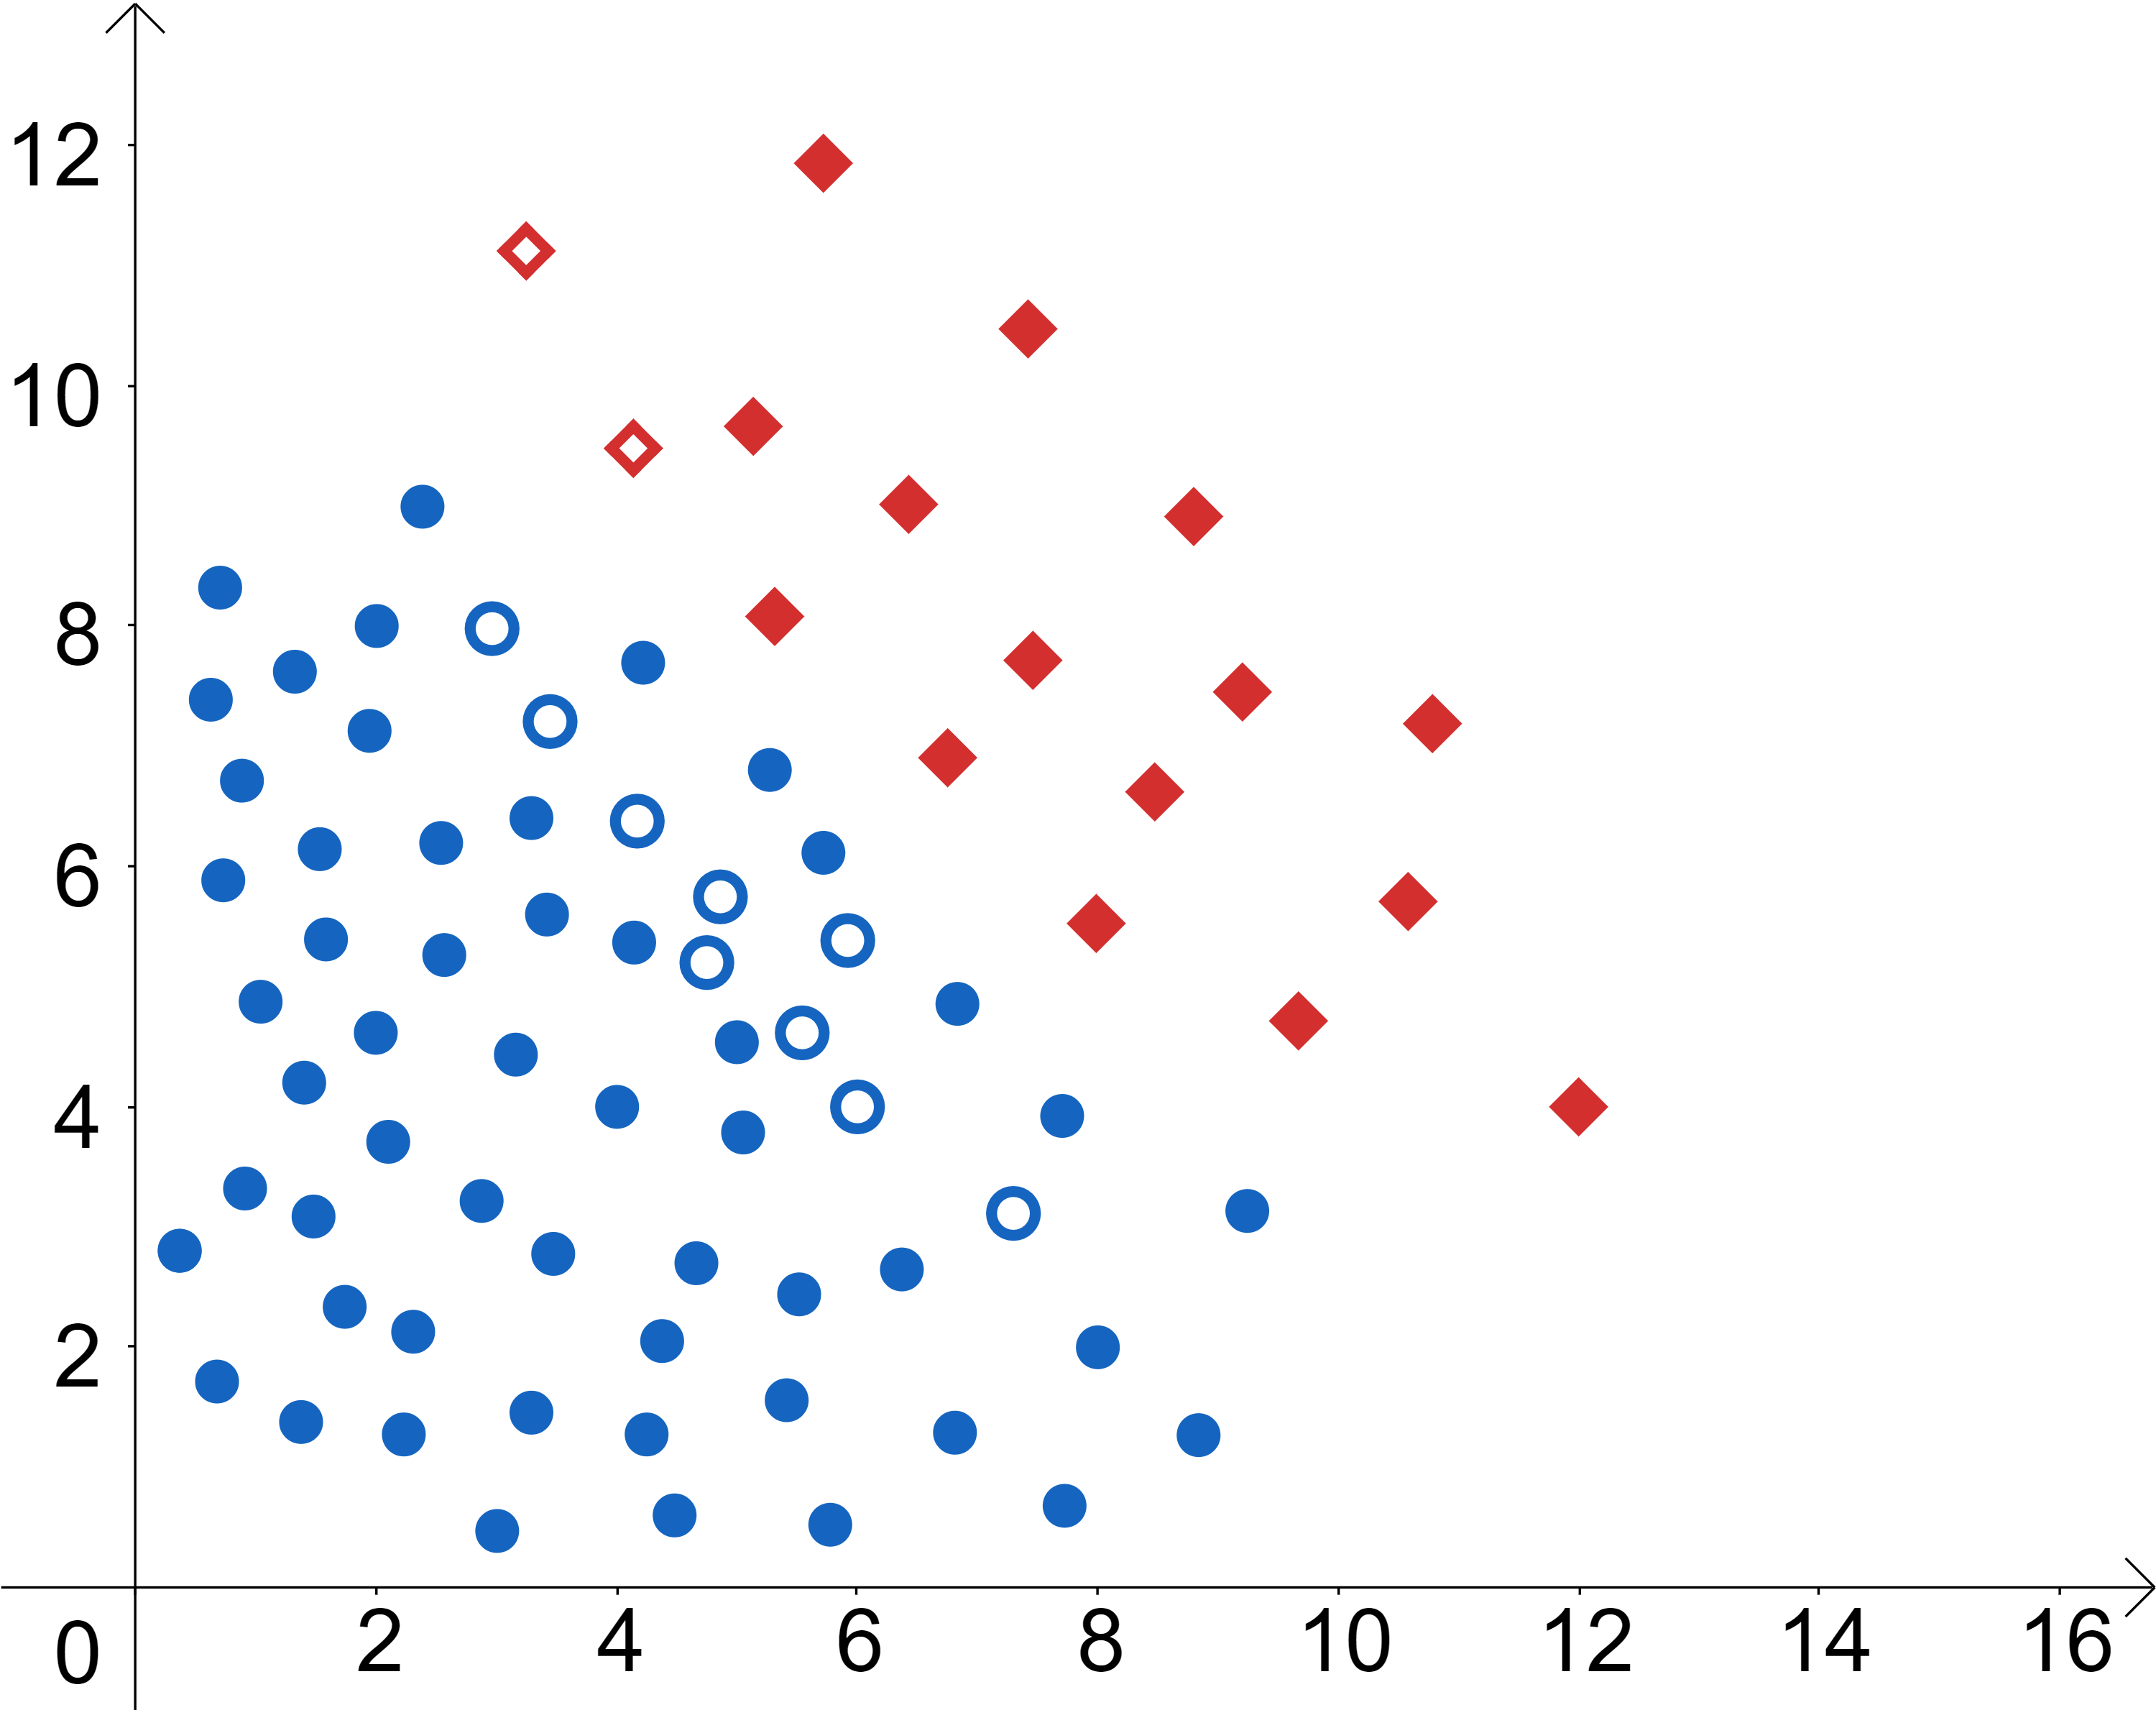
\includegraphics[width=0.9\textwidth]{ADS_Journal/PU figures/final_1.png}\\
  \end{minipage}
  \caption{Expected result of self-training and active learning.}
  \label{fig:expected result}
%   \vspace{0 mm}
\end{figure}

\subsubsection{Final model building}
\label{subsubsubsec:Pre-training}
After labeling enough samples by self-training, we need to build the final model for each new KPI stream using the anomalous samples $setP$, normal samples $setN$, unlabeled samples $setU$, and unlabeled samples of new KPI stream $setU_{new}$. In this work, we adopt CPLE \cite{loog2016contrastive}, an extension model of self-training. There is some overlap between the positive samples and negative samples, so if we use a simple self-training method to label some unlabeled samples, the samples close to the boundary between positive samples and negative samples are prone to be misclassification which will lead to a poor performance of the final model.
Therefore, we use CPLE to build the final model. It is more robust than other semi-supervised learning algorithms because it needs no strong assumptions such as the accurate estimation for data distribution of labeled and unlabeled data.
